\documentclass[a4paper]{article}

% CJK support: prefer ctex, fallback to XeTeX native line breaking
\IfFileExists{ctex.sty}{
  \usepackage[fontset=fandol]{ctex}
}{
  % Fallback for minimal TeX installs (e.g. MacTeX Basic, TeX Live scheme-basic)
  % without ctex/xeCJK. Uses XeTeX's built-in CJK line breaking.
  \usepackage{fontspec}
  \XeTeXlinebreaklocale "zh"
  \XeTeXlinebreakskip = 0pt plus 1pt
  \IfFontExistsTF{Songti SC}{\setmainfont{Songti SC}}{%
    \IfFontExistsTF{Noto Serif CJK SC}{\setmainfont{Noto Serif CJK SC}}{}%
  }
  \IfFontExistsTF{Heiti SC}{\setsansfont{Heiti SC}}{%
    \IfFontExistsTF{Noto Sans CJK SC}{\setsansfont{Noto Sans CJK SC}}{}%
  }
}

% Basic packages
\usepackage{amsmath, amssymb}
\usepackage{graphicx}
\usepackage[margin=2.5cm]{geometry}
\emergencystretch=3em
\usepackage[most]{tcolorbox}
\usepackage{etoolbox}
\usepackage{listings}
\usepackage{hyperref}
\usepackage{booktabs}
\usepackage{array}
\usepackage{subcaption}
\usepackage{float}
\usepackage{tikz}
\IfFileExists{pgfplots.sty}{
    \usepackage{pgfplots}
    \pgfplotsset{compat=1.18}
}{}

% ===== Highlight boxes =====
\newtcolorbox{knowledgebox}[1]{
    enhanced, colback=blue!5!white, colframe=blue!75!black, colbacktitle=blue!75!black,
    coltitle=white, fonttitle=\bfseries, title={#1}, attach boxed title to top left={yshift=-2mm, xshift=2mm},
    boxrule=1pt, sharp corners
}

\newtcolorbox{importantbox}[1]{
    enhanced, colback=yellow!10!white, colframe=yellow!80!black, colbacktitle=yellow!80!black,
    coltitle=black, fonttitle=\bfseries, title={#1}, sharp corners
}

\newtcolorbox{warningbox}[1]{
    enhanced, colback=red!5!white, colframe=red!75!black, colbacktitle=red!75!black,
    coltitle=white, fonttitle=\bfseries, title={#1}, sharp corners
}

\newtcolorbox{practicebox}[1]{
    enhanced, colback=black!3!white, colframe=black!75, colbacktitle=black!75,
    coltitle=white, fonttitle=\bfseries, title={#1}, sharp corners
}

% ===== Code listings =====
\lstset{
    basicstyle=\ttfamily\small,
    keywordstyle=\color{blue},
    stringstyle=\color{red!60!black},
    commentstyle=\color{green!60!black},
    breaklines=true,
    frame=single,
    numbers=left,
    numberstyle=\tiny\color{gray},
    captionpos=b,
    extendedchars=false
}

% ===== Figure provenance and unit macros =====
% \vtag goes inside \caption{...}; \srcnote{MM:SS--MM:SS} follows the figure environment.
\newcommand{\vtag}{\protect\footnotemark}
\newcommand{\srcnote}[1]{\footnotetext{视频画面时间区间：#1。若为裁剪图，时间区间仍对应原视频画面。}}
% Units work in text and math mode; never hand-write $^\circ$ or \AA inside \mathrm.
\newcommand{\degC}{\ensuremath{^{\circ}\mathrm{C}}}
\newcommand{\um}{\ensuremath{\mu\mathrm{m}}}
\newcommand{\nm}{\ensuremath{\mathrm{nm}}}
\newcommand{\angstrom}{\ensuremath{\text{\AA}}}

% ===== Front-page metadata =====
% Fill these in when generating notes.
\newcommand{\notetitle}{概率论（二）}
\newcommand{\notesubtitle}{GAMES001 图形学中的数学 · 第 9 集：噪声、蒙特卡洛积分与随机采样}
\newcommand{\noteauthors}{根据 GAMES-Webinar 直播录像整理（倪星宇 主讲）}
\newcommand{\notedate}{2024年5月13日（直播）}
\newcommand{\videochannel}{GAMES-Webinar（哔哩哔哩）}
\newcommand{\videopublishdate}{2024年3月6日（合集）}
\newcommand{\videoduration}{1小时8分14秒}
\newcommand{\videourl}{https://www.bilibili.com/video/BV1MF4m1V7e3/?p=9}
\newcommand{\videocoverpath}{cover.jpg}

\begin{document}

% ===== Title page =====
\begin{titlepage}
\centering
{\Large 课程笔记\par}
\vspace{1.2cm}
{\huge\bfseries \notetitle\par}
\ifdefempty{\notesubtitle}{}{
\vspace{0.3cm}
{\large \notesubtitle\par}
}
\vspace{0.5cm}
{\large \noteauthors\par}
\vspace{0.3cm}
{\large \notedate\par}
\vspace{1.0cm}

\ifdefempty{\videocoverpath}{
{\small 请在生成笔记时填入视频封面图的本地路径。\par}
}{
\includegraphics[width=0.82\textwidth,height=0.40\textheight,keepaspectratio]{\videocoverpath}\par
}

\vfill
\begin{tcolorbox}[width=0.9\textwidth, colback=black!2!white, colframe=black!60, sharp corners]
\textbf{视频作者/频道}：\videochannel\par
\textbf{发布日期}：\videopublishdate\par
\textbf{视频时长}：\videoduration\par
\textbf{视频链接}：
\ifdefempty{\videourl}{
未填写
}{
\href{\videourl}{\nolinkurl{\videourl}}
}
\end{tcolorbox}
\end{titlepage}

\tableofcontents
\newpage

%% --- 正文内容开始 --- %%

\section{这一讲讲什么}

第九讲由倪星宇主讲，是概率论的第二讲。假期回来，讲者先用几分钟回顾了上一讲的内容：概率的定义、古典概型、条件概率、随机变量及其分布，期望、方差、协方差和矩，以及大数定律（弱大数定律即辛钦大数定律、伯努利大数定律）和中心极限定理。上一讲是概率论最基础的知识，这一讲要回答的问题是：概率论在图形学当中到底有什么用。

本讲有三部分：第一部分是噪声，从声音的“颜色”讲到图像处理中的抖动；第二部分是蒙特卡洛积分，包括收敛性、重要性采样和拟蒙特卡洛法；第三部分是随机数的变换，讨论如何在单位球面上均匀采样。

\begin{importantbox}{本讲的主线}
图形学里的随机性有两种用法。一种是把随机“加进”结果里，让人眼看起来更自然，例如用噪声做抖动；另一种是用随机样本去“估计”一个确定的量，例如用蒙特卡洛方法算积分。两种用法都关心同一个问题：样本分布得是否均匀、它的频谱长什么样。所以本讲会反复出现白噪声、蓝噪声和低差异序列。
\end{importantbox}

\section{噪声的“颜色”}

\subsection{从光的颜色说起}

讲者说，大家可能会奇怪：“噪声”听起来是声学里的概念，它和概率之间怎么建立联系？他先从颜色讲起。颜色是人眼对不同波长的光的混合的感知。比如日光看起来是白色，但它其实是红橙黄绿青蓝紫各种波长的光的混合，所以颜色并不只对应一种波长。每一种频谱对应于一种颜色，但不同的频谱可能对应于相同的颜色。

\noindent\begin{minipage}{\textwidth}
\begin{figure}[H]
\centering
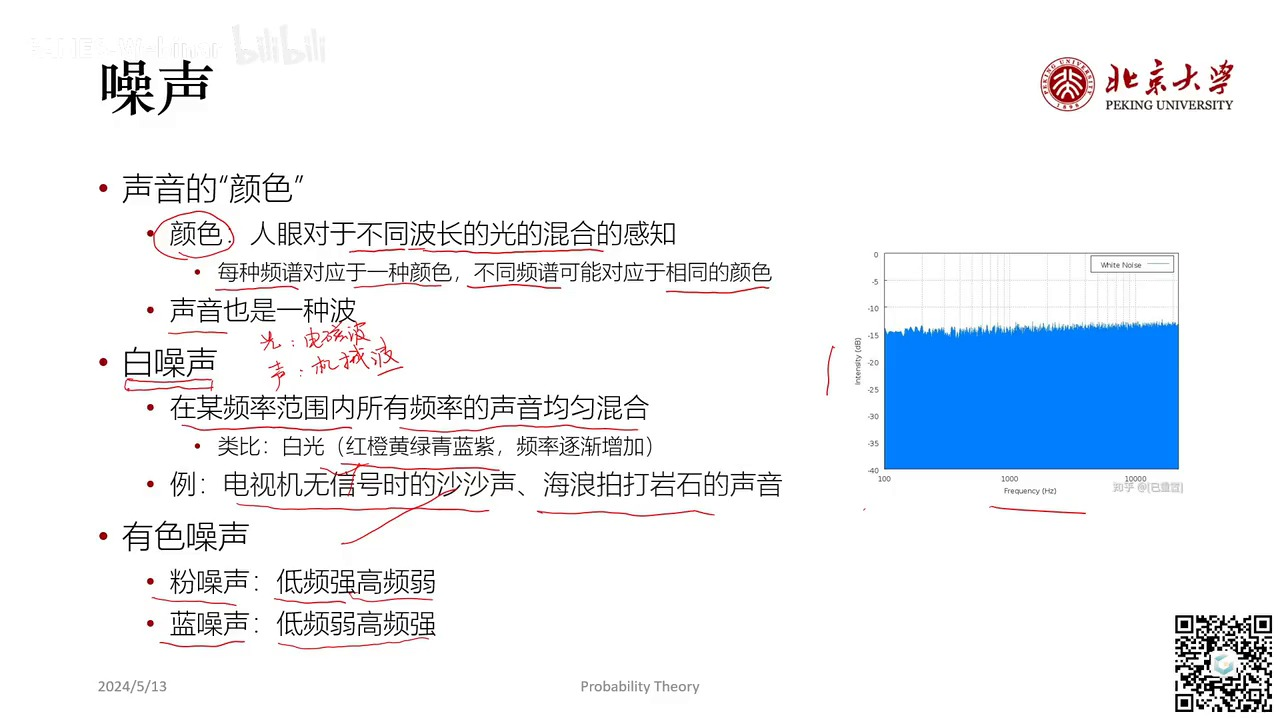
\includegraphics[width=0.92\textwidth]{figures/fig_01_noise_color.jpg}
\caption{声音的“颜色”：白噪声与有色噪声，右侧为白噪声的频谱\vtag}
\end{figure}
\srcnote{00:06:15--00:06:30}
\end{minipage}


声音和光一样也是一种波，只不过光是电磁波，声音是机械波。既然光的频谱可以对应颜色，声音的频谱也可以借用颜色来命名。

\subsection{白噪声与有色噪声}

白噪声是在某频率范围内所有频率的声音均匀混合。它可以类比白光：白光里红橙黄绿青蓝紫频率逐渐增加，各种频率都有。例子是电视机无信号时的沙沙声，以及海浪拍打岩石的声音。这些声音不是以乐音的方式给出的，所以称为噪声。

有色噪声则是各频率强度不均匀。粉噪声的频谱偏向左侧，即低频强、高频弱；蓝噪声则相反，低频弱、高频强。

\begin{knowledgebox}{为什么叫粉色和蓝色}
讲义作者补充：在可见光中，红光频率低、蓝光频率高。低频强的噪声好比偏红的光，所以叫“粉”（介于白与红之间）；高频强的噪声好比偏蓝的光，所以叫“蓝”。命名完全是类比可见光的频谱，与真实颜色无关。
\end{knowledgebox}

\subsection{图像中的随机噪声}

\noindent\begin{minipage}{\textwidth}
\begin{figure}[H]
\centering
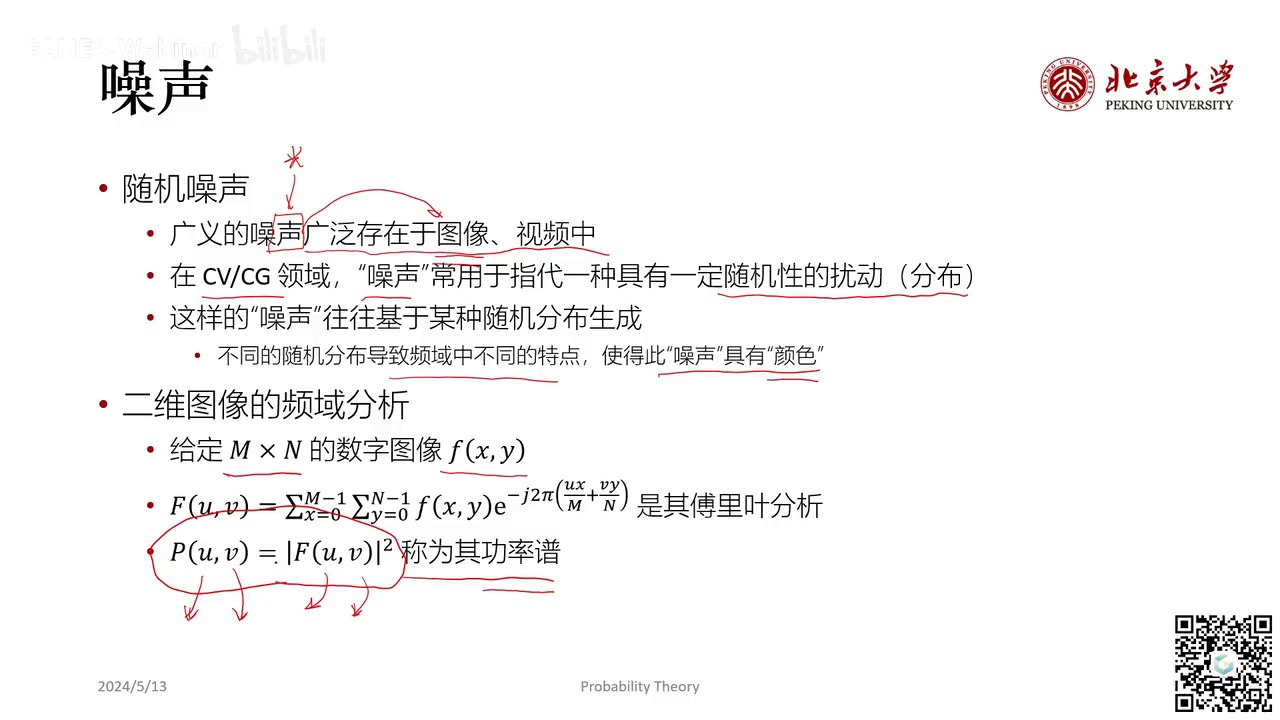
\includegraphics[width=0.92\textwidth]{figures/fig_02_noise_image.jpg}
\caption{随机噪声的概念与二维图像的频域分析\vtag}
\end{figure}
\srcnote{00:08:45--00:09:00}
\end{minipage}


在更广的意义上，噪声广泛存在于图像和视频中。在计算机视觉和图形学领域，“噪声”常用于指代一种具有一定随机性的扰动，或者说服从某种随机分布。这样的噪声往往基于某种随机分布生成；不同的随机分布导致频域中不同的特点，使得这些“噪声”具有“颜色”。

对二维图像也可以做频域分析。给定 $M\times N$ 的数字图像 $f(x,y)$，它的二维离散傅里叶变换为
\begin{equation}
F(u,v)=\sum_{x=0}^{M-1}\sum_{y=0}^{N-1}f(x,y)\,e^{-j2\pi\left(\frac{ux}{M}+\frac{vy}{N}\right)},
\end{equation}
$P(u,v)=|F(u,v)|^2$ 称为它的功率谱。这里的 $u,v$ 是与频率对应的参量。讲者说，这部分只需要概念性地理解，并不需要真的掌握如何对数字图像做傅里叶分析；第七讲已经介绍了傅里叶变换。

\section{图像的量化与抖动}

\subsection{量化问题}

\noindent\begin{minipage}{\textwidth}
\begin{figure}[H]
\centering
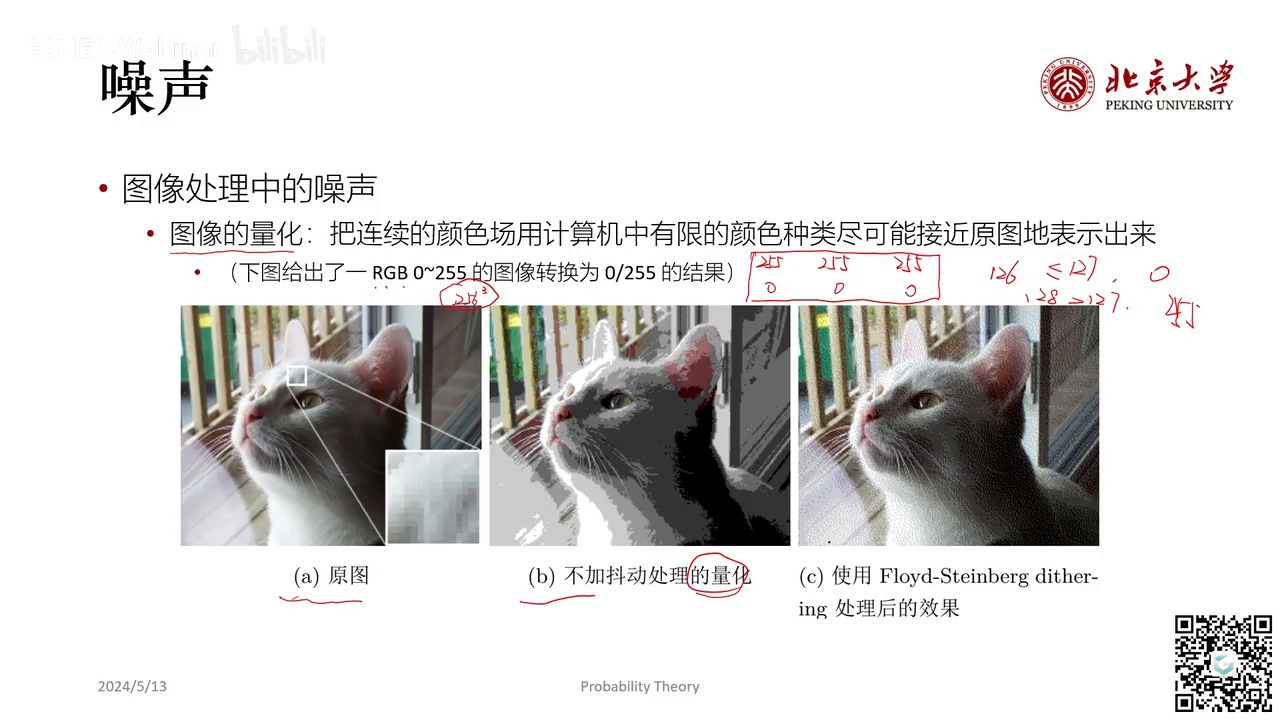
\includegraphics[width=0.92\textwidth]{figures/fig_03_quantize.jpg}
\caption{图像的量化：原图、不加抖动的量化与 Floyd--Steinberg 抖动\vtag}
\end{figure}
\srcnote{00:11:30--00:11:45}
\end{minipage}


讲者接着讲了一个经典问题：图像的量化。现在的显示技术中，红、绿、蓝每个通道一般有 $0$ 到 $255$ 共 $256$ 种取值，总共形成 $256^3$ 种颜色。这个数相当大，所以我们一般把颜色空间看成连续的。但假如显示设备支持不了这么好的显示，比如每个像素只能显示 0 或 255，怎样显示的结果才最接近原图？

所谓量化，就是把连续的颜色场用计算机中有限的颜色种类尽可能接近原图地表示出来。课件中图 (a) 是原图，(b) 是直接量化的结果：亮度低于一半的置为 0，否则置为 255。可以发现 (b) 相对于 (a) 丢失了非常多的细节。(c) 同样只用 0 和 255 两种值，但使用了 Floyd--Steinberg 抖动处理，看起来接近原图得多。本节要讨论如何达到 (c) 的效果。

\subsection{两种非随机方案}

\noindent\begin{minipage}{\textwidth}
\begin{figure}[H]
\centering
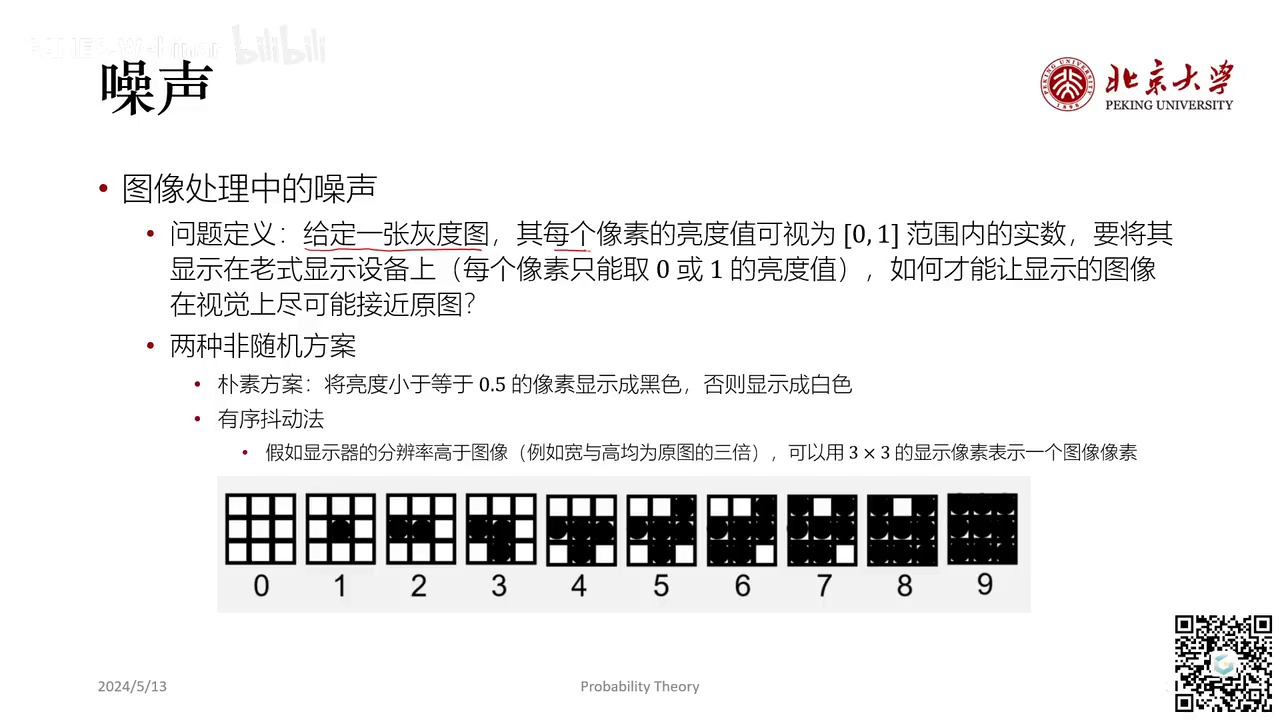
\includegraphics[width=0.92\textwidth]{figures/fig_04_dither_def.jpg}
\caption{问题定义与两种非随机方案：朴素方案与有序抖动法\vtag}
\end{figure}
\srcnote{00:12:00--00:12:15}
\end{minipage}


把问题简化：给定一张灰度图，每个像素的亮度值可视为 $[0,1]$ 范围内的实数，$0$ 最暗，$1$ 最亮。要把它显示在老式显示设备上，每个像素只能取 0 或 1 的亮度值，如何才能让显示的图像在视觉上尽可能接近原图？

朴素方案是：亮度小于等于 $0.5$ 的像素显示成黑色，否则显示成白色。这就是前面的直接量化。

另一种思路是有序抖动法。假如显示器的分辨率高于图像，例如原图是 $100\times 100$，显示器是 $300\times 300$，显示器每个像素只能取 0 或 1。这时可以用 $3\times 3$ 的显示像素来表示一个图像像素：把几个像素放在一起，就有了更多种显示能力。比如原图像素亮度为 $0.5$，就让 $3\times 3$ 的显示像素中大约一半被点亮，从远处看就接近中等灰度。$3\times 3$ 阵列中点亮的个数可以是 $0$ 到 $9$，对应 $0,1/9,2/9,\dots,1$ 十个灰度等级，原图亮度更接近哪个等级，就用哪种图案。

\noindent\begin{minipage}{\textwidth}
\begin{figure}[H]
\centering
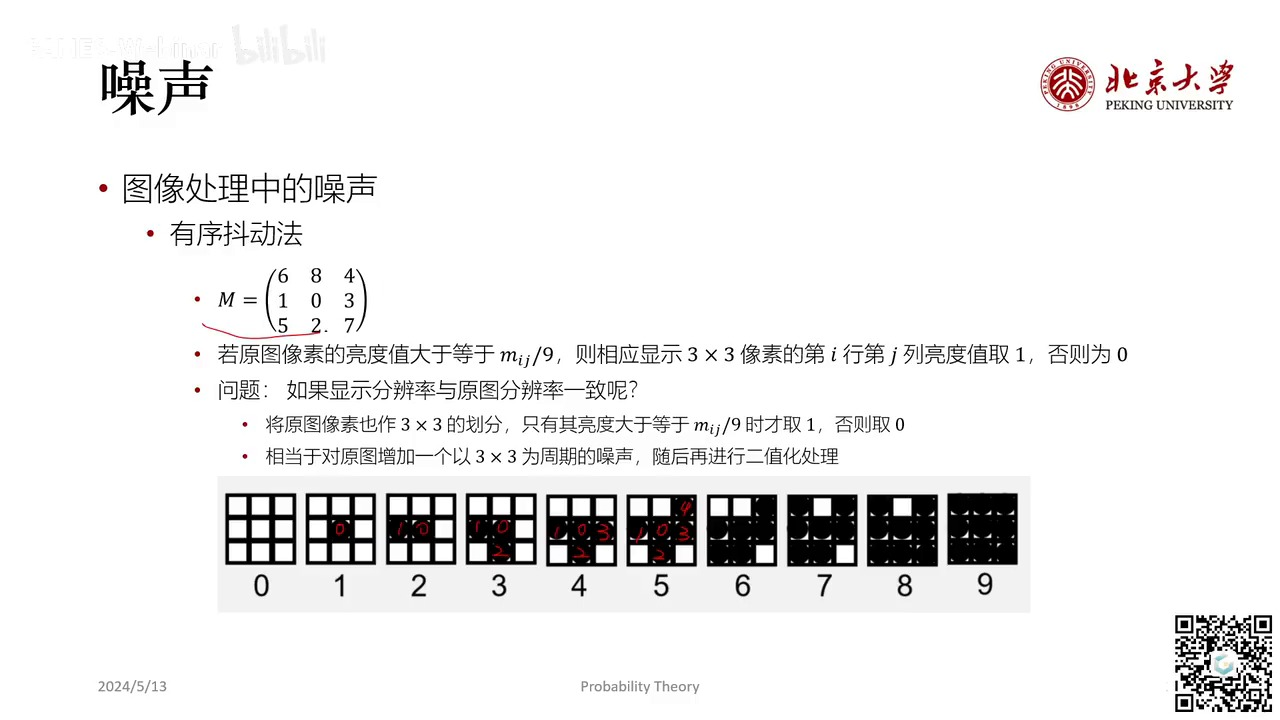
\includegraphics[width=0.92\textwidth]{figures/fig_05_dither_matrix.jpg}
\caption{有序抖动矩阵 $M$ 及其对应的十种点亮图案\vtag}
\end{figure}
\srcnote{00:16:30--00:16:45}
\end{minipage}


点亮的顺序由一个矩阵给出
\begin{equation}
M=\begin{pmatrix}6&8&4\\1&0&3\\5&2&7\end{pmatrix}.
\end{equation}
讲者解释：最先填上颜色的是中间，所以标成 0；第二个填上的是最左边，标成 1；依此类推。规则写成：若原图像素的亮度值大于等于 $m_{ij}/9$，则对应的 $3\times 3$ 显示像素中第 $i$ 行第 $j$ 列的亮度取 1，否则取 0。

\subsection{分辨率一致时的有序抖动}

如果显示分辨率与原图分辨率一致呢？做法是把原图像素也作 $3\times 3$ 的划分，只有其亮度大于等于 $m_{ij}/9$ 时才取 1，否则取 0。讲者在原图上把像素分成若干块，每块都是 $3\times 3$ 的阵列，直接比较它在阵列中的第几行第几列，与对应的 $m_{ij}/9$ 比较。

\begin{knowledgebox}{有序抖动 = 加周期噪声再二值化}
讲者指出这件事的本质：原来是看像素亮度是否大于等于 $0.5$，现在是看它是否大于等于 $m_{ij}/9$。这相当于对原图叠加了一个以 $3\times 3$ 为周期的“噪声”，随后再进行二值化处理。阈值不再是常数，而是在空间上周期变化的。
\end{knowledgebox}

\noindent\begin{minipage}{\textwidth}
\begin{figure}[H]
\centering
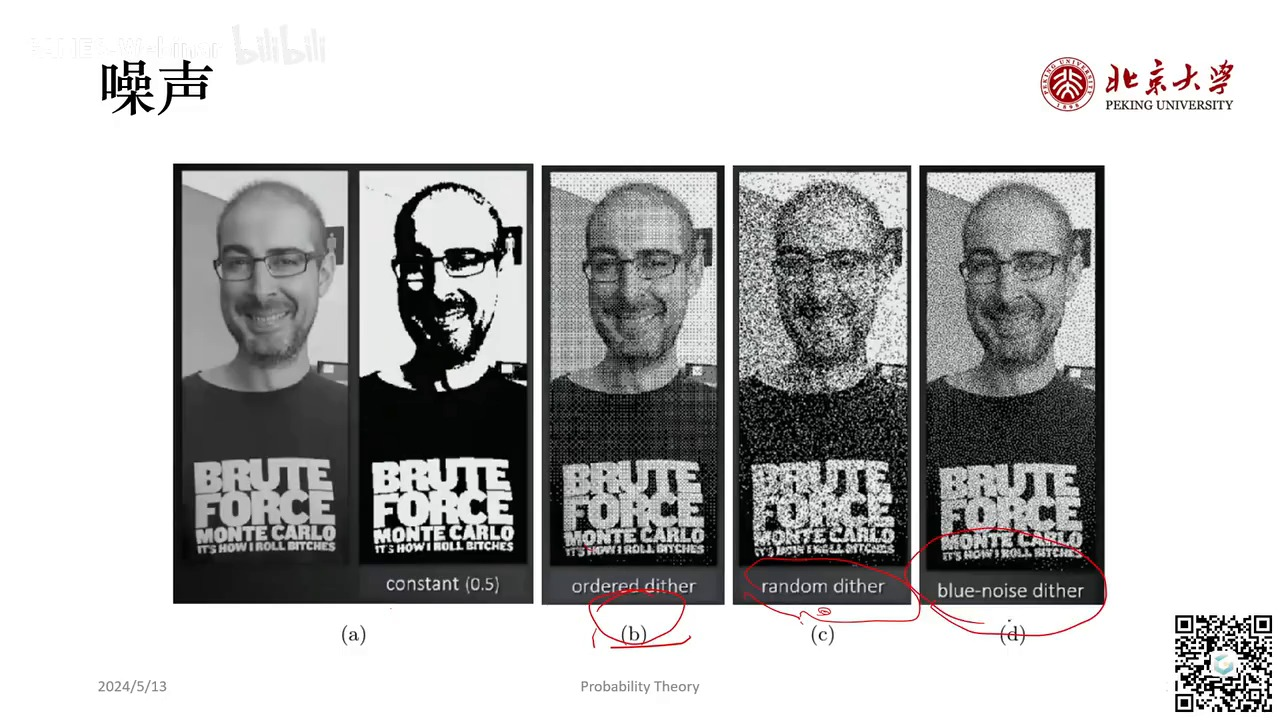
\includegraphics[width=0.92\textwidth]{figures/fig_06_dither_compare.jpg}
\caption{四种方案的对比：常数阈值、有序抖动、随机抖动与蓝噪声抖动\vtag}
\end{figure}
\srcnote{00:21:00--00:21:15}
\end{minipage}


课件对比了四种方案的效果。(a) 是原图；(b) 是常数阈值 $0.5$，效果也很有艺术感，但丢失了非常多的细节，根本看不清人物的面部特征；(c) 是有序抖动，已经能看清一点面部特征了；(d) 是在每个像素上随机加一个值后再二值化的随机抖动；最后一幅用蓝噪声抖动，效果最好。

\section{基于噪声的抖动}

\subsection{随机抖动的数学描述}

\noindent\begin{minipage}{\textwidth}
\begin{figure}[H]
\centering
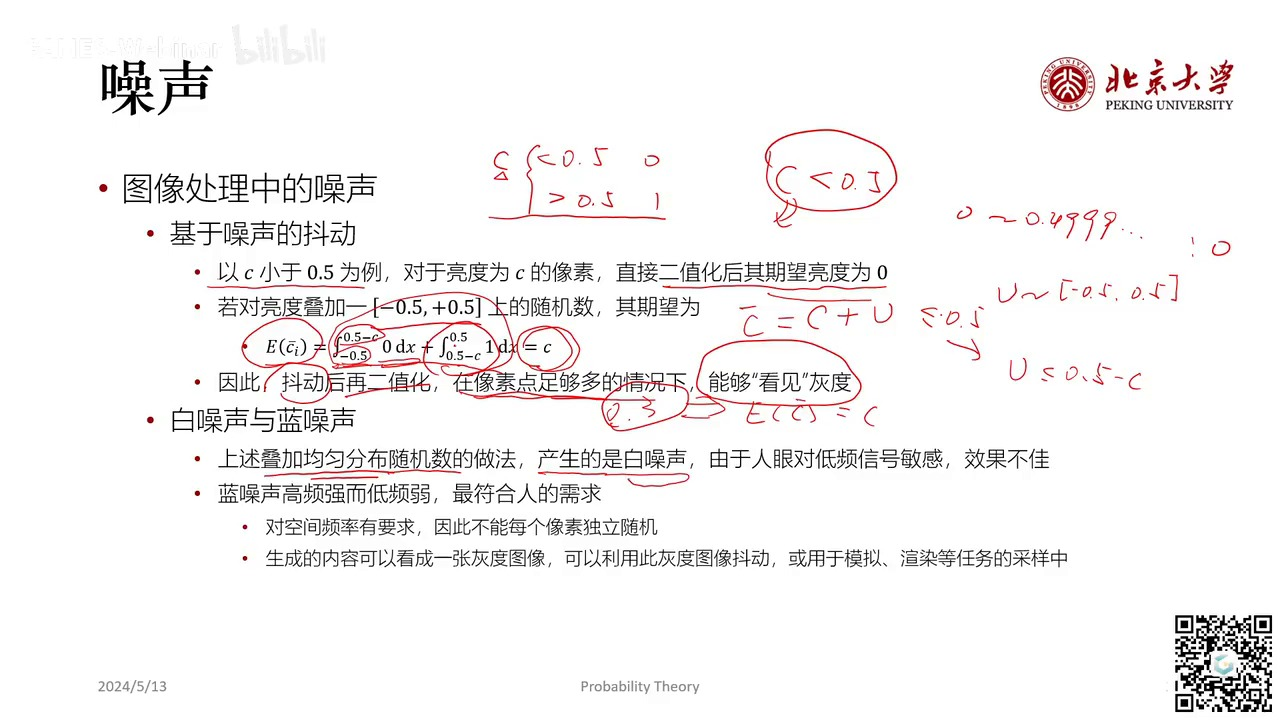
\includegraphics[width=0.92\textwidth]{figures/fig_07_noise_dither.jpg}
\caption{基于噪声的抖动：期望分析，以及白噪声与蓝噪声\vtag}
\end{figure}
\srcnote{00:26:15--00:26:30}
\end{minipage}


讲者用数学来描述随机抖动做了什么。如果不抖动，直接判断：某像素亮度为 $c$，以 $c<0.5$ 为例，不管 $c$ 出现在图片上的什么地方，也不管哪一次去量化，都会被直接置为 0，所以其期望亮度为 0，信息完全丢失。

若对亮度叠加一个 $[-0.5,+0.5]$ 上的随机数 $U$，即把 $c$ 变成 $c+U$ 再二值化。当 $U<0.5-c$ 时结果为 0，当 $U$ 从 $0.5-c$ 到 $0.5$ 时结果为 1。由于 $U$ 是均匀分布，概率密度处处为 1，于是二值化结果 $\bar c$ 的期望为
\begin{equation}
E(\bar c)=\int_{-0.5}^{0.5-c}0\,\mathrm{d}x+\int_{0.5-c}^{0.5}1\,\mathrm{d}x=c .
\end{equation}

\noindent\begin{minipage}{\textwidth}
\begin{figure}[H]
\centering
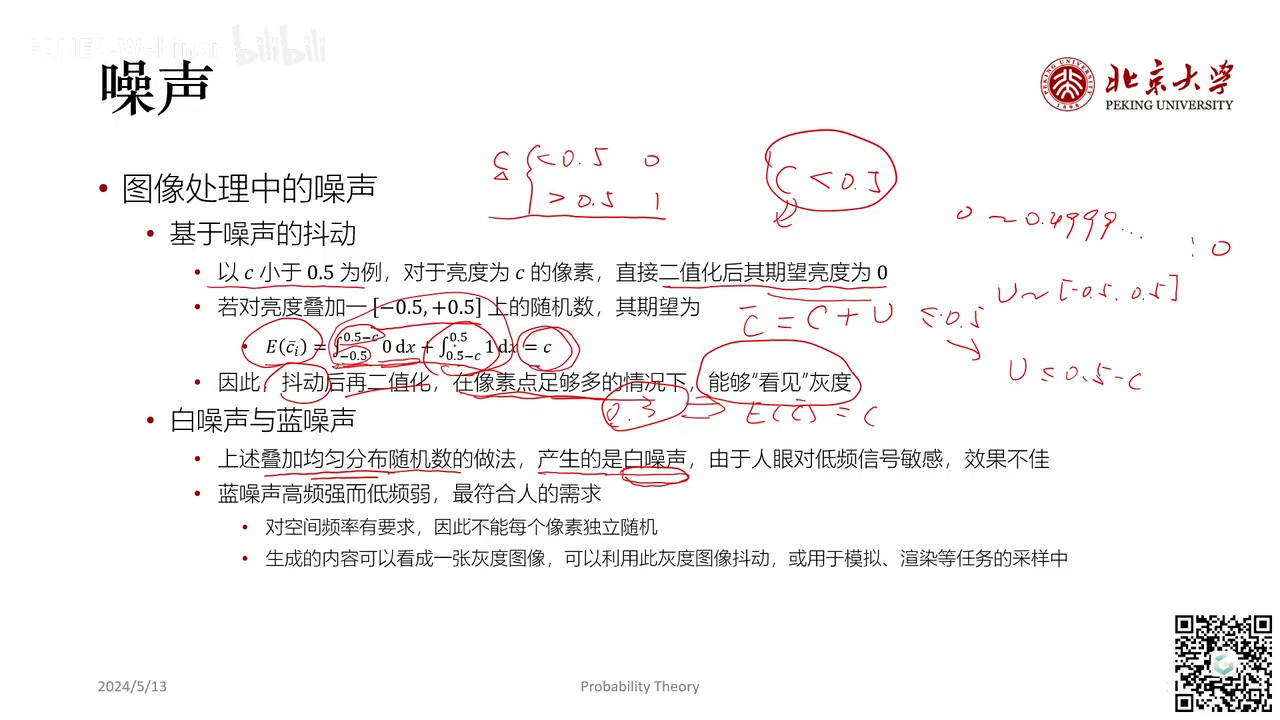
\includegraphics[width=0.92\textwidth]{figures/fig_08_noise_dither_note.jpg}
\caption{讲者在课件上演算随机抖动的期望\vtag}
\end{figure}
\srcnote{00:27:00--00:27:15}
\end{minipage}


因此，抖动后再二值化，在像素点足够多的情况下，能够“看见”灰度。讲者举例：亮度为 $0.3$ 的像素可能在图片中很多地方出现，二值化后它们有的取 0、有的取 1，但在随机意义下，它们的期望仍然是 $0.3$。

\begin{importantbox}{抖动为什么有效}
直接量化是一个确定的、有偏的操作，期望亮度和原亮度不同；加入均匀噪声后，每个像素的二值结果变成随机变量，而它的期望恰好等于原亮度，是无偏的。人眼会对一片区域做平均，相当于对大量样本取平均，于是看到的就接近原灰度。这正是上一讲大数定律的一个直观应用。
\end{importantbox}

\subsection{白噪声与蓝噪声}

上述做法每个像素独立叠加均匀分布的随机数，对它做傅里叶分析，频谱在各个频率上的强度大致相同，所以相当于在原图上加了白噪声。由于人眼对低频信号敏感、对高频信号不敏感，白噪声中的低频成分会被看成斑块，效果不佳。

蓝噪声的高频强、低频弱，从人的观感上来说最符合需求。但它的生成就没那么简单：蓝噪声对空间频率有要求，因此不能每个像素独立随机。要生成满足蓝噪声的分布需要特定的算法，讲者说这超出了本课程的框架，感兴趣可以自己去看图形学中生成蓝噪声的方法。生成的内容可以看成一张灰度图像，可以利用此灰度图像抖动，也可用于模拟、渲染等任务的采样中。讲者还预告：从某种意义上说，蓝噪声生成的序列就是后面要讲的低差异序列。

\begin{warningbox}{“随机”不等于“均匀”}
独立随机撒点时，点与点之间可能挨得很近，也可能留下大片空白，这些低频的起伏正是白噪声的特征。想要“既随机又均匀”，必须让样本之间相互关联，比如蓝噪声或低差异序列。这一点在下面的拟蒙特卡洛法中还会遇到。
\end{warningbox}

\section{蒙特卡洛积分}

\subsection{基本案例：求不规则图形的面积}

\noindent\begin{minipage}{\textwidth}
\begin{figure}[H]
\centering
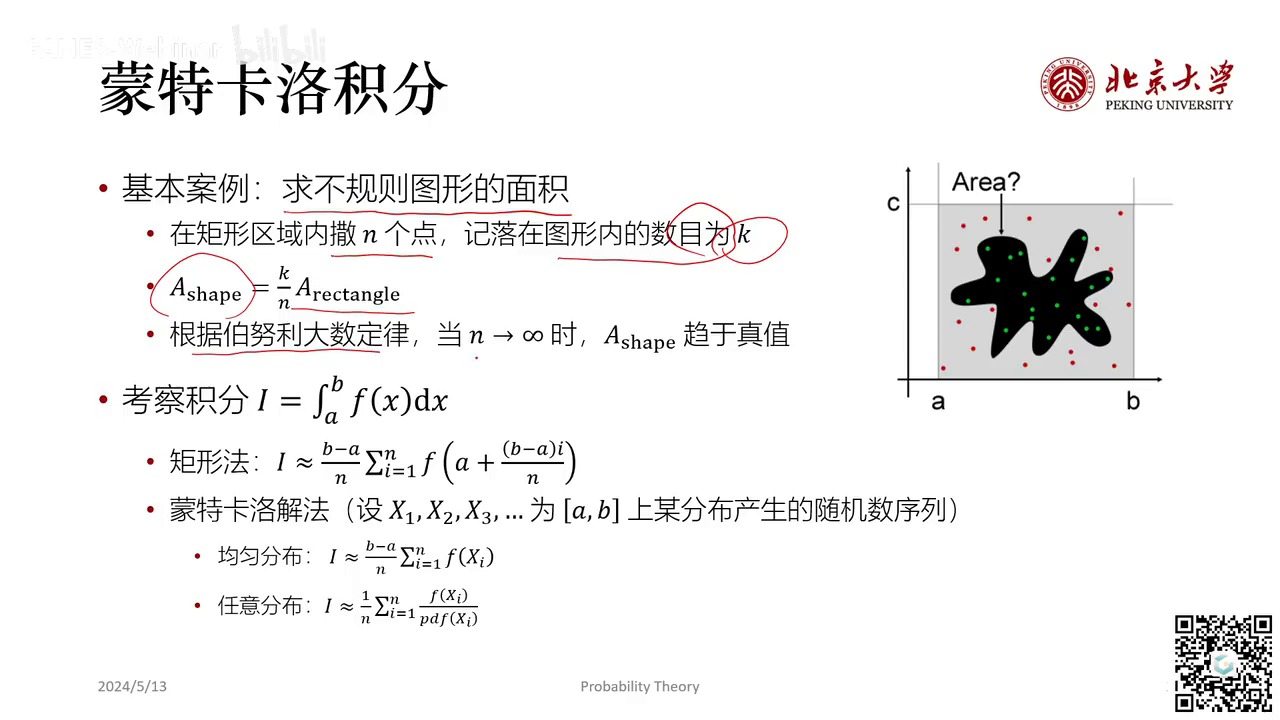
\includegraphics[width=0.92\textwidth]{figures/fig_09_mc_area.jpg}
\caption{蒙特卡洛积分的基本案例：撒点求不规则图形的面积，以及积分的矩形法与蒙特卡洛解法\vtag}
\end{figure}
\srcnote{00:30:30--00:30:45}
\end{minipage}


在概率论中，最经典的例子是用蒙特卡洛方法求不规则图形的面积。先在包含图形的矩形区域内随机撒 $n$ 个点，记落在图形内的点数为 $k$，则
\begin{equation}
A_{\text{shape}}\approx\frac{k}{n}A_{\text{rectangle}} .
\end{equation}
根据伯努利大数定律，当 $n\to\infty$ 时，$A_{\text{shape}}$ 趋于真值。

\subsection{用随机数求定积分}

考察积分 $I=\int_a^b f(x)\,\mathrm{d}x$。最简单的做法是矩形法：把 $[a,b]$ 分成 $n$ 段，每段取一个函数值，乘以每段长度 $(b-a)/n$ 再求和：
\begin{equation}
I\approx\frac{b-a}{n}\sum_{i=1}^{n}f\!\left(a+\frac{(b-a)i}{n}\right).
\end{equation}
蒙特卡洛解法则用随机数：设 $X_1,X_2,X_3,\dots$ 为 $[a,b]$ 上某分布产生的随机数序列。若是均匀分布，
\begin{equation}
I\approx\frac{b-a}{n}\sum_{i=1}^{n}f(X_i).
\end{equation}
讲者的直观解释：随便取一点，用该点的函数值乘以 $b-a$，就当整个区间上的值都等于它，这当然不对；那就再取一点，多取一些点平均起来。

\noindent\begin{minipage}{\textwidth}
\begin{figure}[H]
\centering
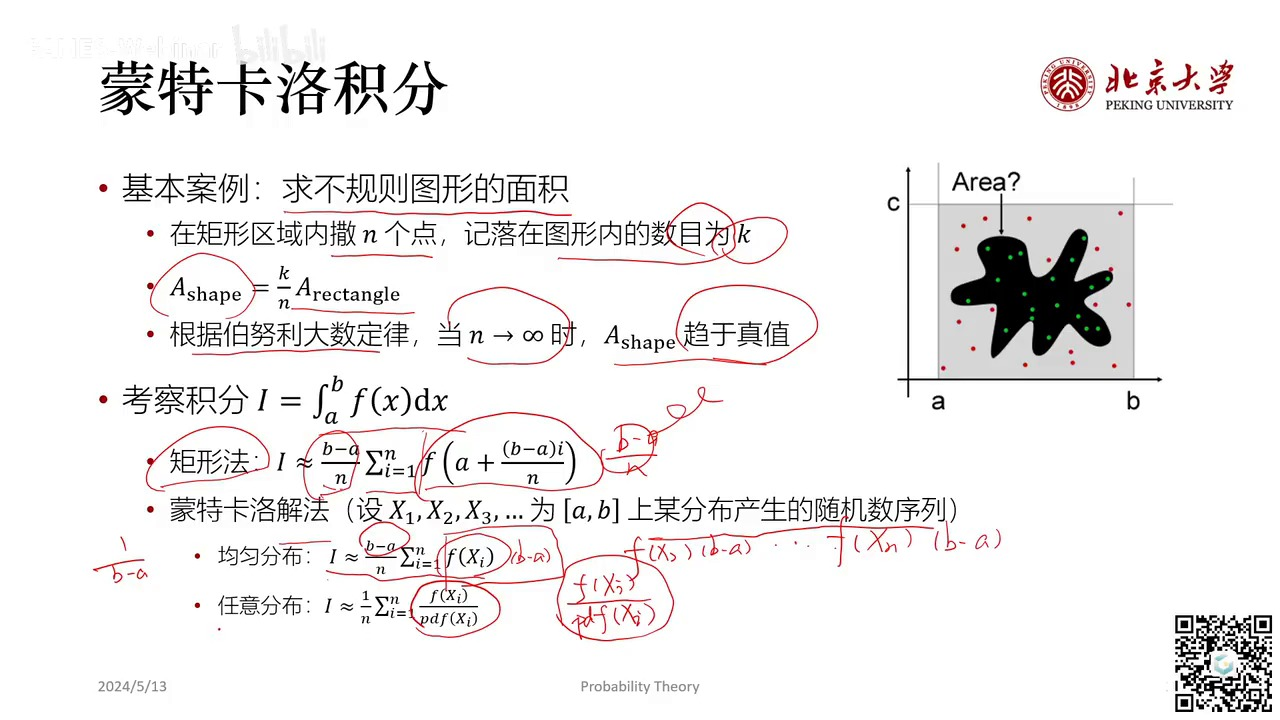
\includegraphics[width=0.92\textwidth]{figures/fig_10_mc_area_note.jpg}
\caption{讲者把均匀分布的概率密度 $1/(b-a)$ 写进公式\vtag}
\end{figure}
\srcnote{00:33:45--00:34:00}
\end{minipage}


若随机数不是均匀分布而是任意分布呢？讲者指出，均匀分布的概率密度函数是 $1/(b-a)$，上式中的 $b-a$ 其实就是把概率密度除掉了。推广到任意概率密度 $\mathrm{pdf}(x)$：
\begin{equation}
I\approx\frac{1}{n}\sum_{i=1}^{n}\frac{f(X_i)}{\mathrm{pdf}(X_i)} .
\end{equation}

\subsection{收敛性证明}

\noindent\begin{minipage}{\textwidth}
\begin{figure}[H]
\centering
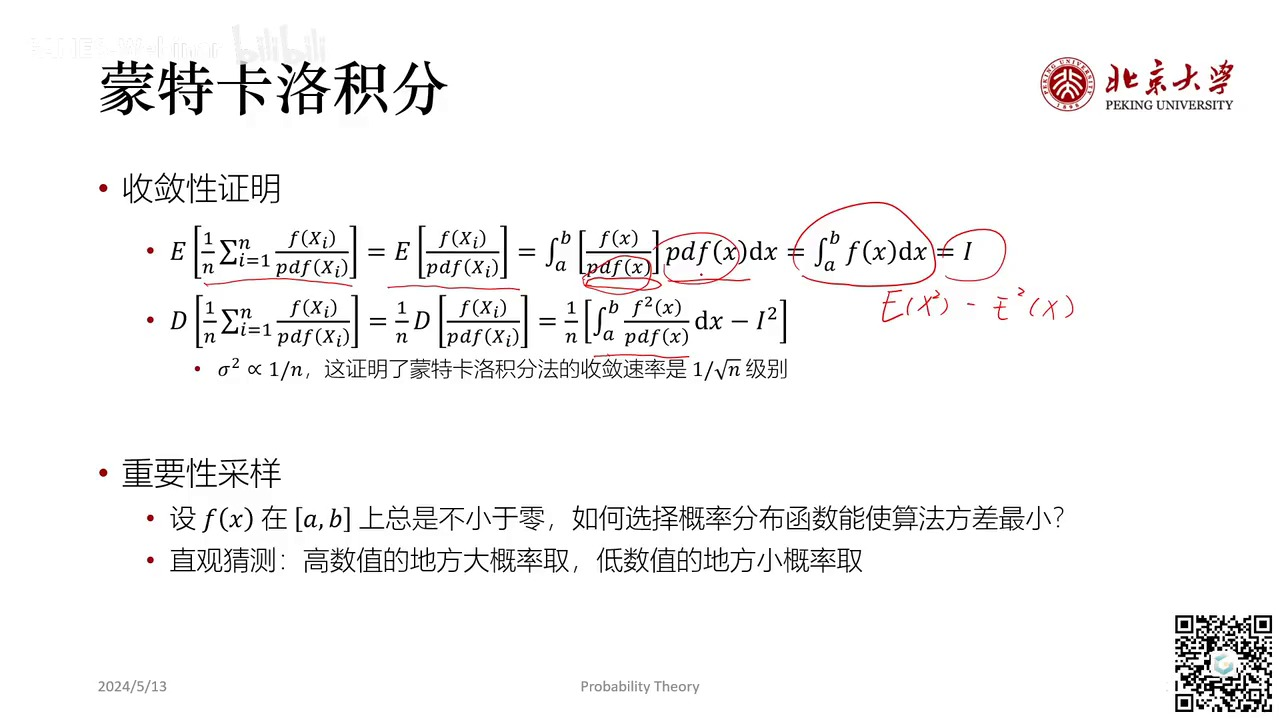
\includegraphics[width=0.92\textwidth]{figures/fig_11_mc_convergence.jpg}
\caption{蒙特卡洛积分的收敛性证明与重要性采样的问题\vtag}
\end{figure}
\srcnote{00:35:45--00:36:00}
\end{minipage}


由于 $X_1,\dots,X_n$ 都是在同一概率分布下抽取的，估计量的期望为
\begin{equation}
E\left[\frac{1}{n}\sum_{i=1}^{n}\frac{f(X_i)}{\mathrm{pdf}(X_i)}\right]=E\left[\frac{f(X)}{\mathrm{pdf}(X)}\right]=\int_a^b\frac{f(x)}{\mathrm{pdf}(x)}\mathrm{pdf}(x)\,\mathrm{d}x=I,
\end{equation}
所以估计是无偏的。再看方差：利用方差的性质，常数 $1/n$ 提出来时要平方成 $1/n^2$，而 $n$ 个独立同分布项的方差之和是 $n$ 倍，于是
\begin{equation}
D\left[\frac{1}{n}\sum_{i=1}^{n}\frac{f(X_i)}{\mathrm{pdf}(X_i)}\right]=\frac{1}{n}D\left[\frac{f(X)}{\mathrm{pdf}(X)}\right]=\frac{1}{n}\left[\int_a^b\frac{f^2(x)}{\mathrm{pdf}(x)}\mathrm{d}x-I^2\right].
\end{equation}

\noindent\begin{minipage}{\textwidth}
\begin{figure}[H]
\centering
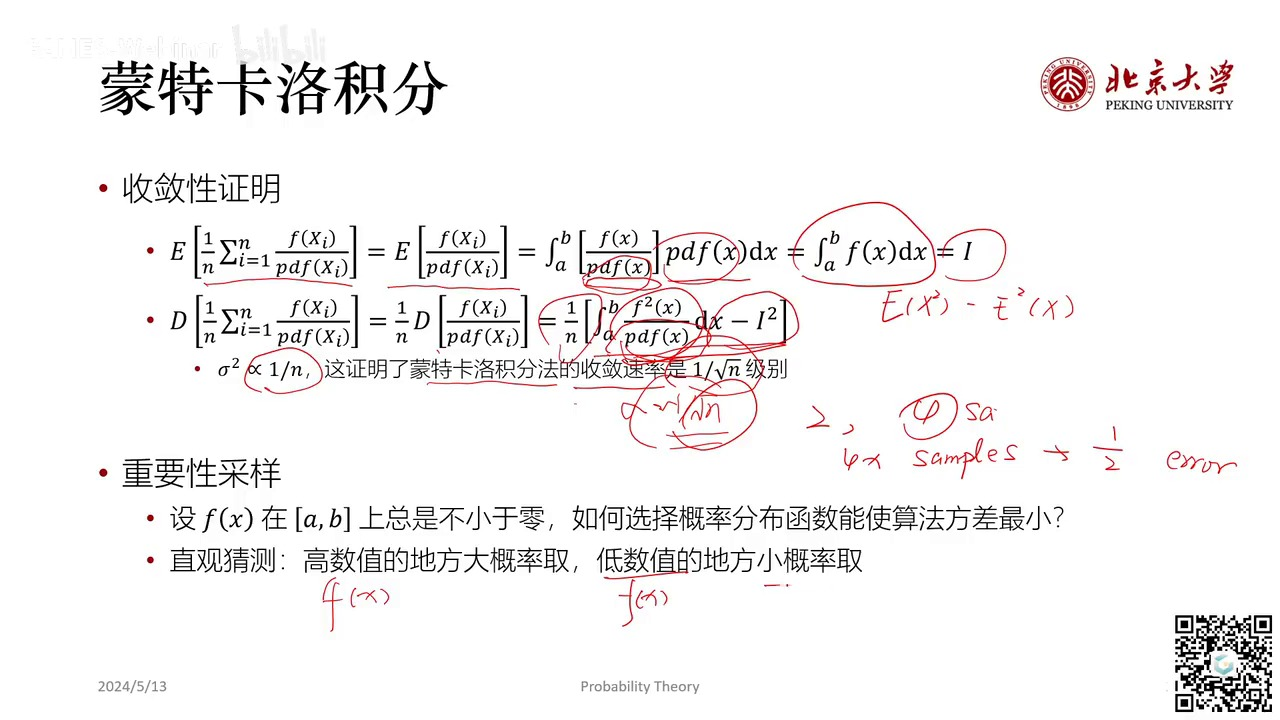
\includegraphics[width=0.92\textwidth]{figures/fig_12_mc_convergence_note.jpg}
\caption{讲者在方差推导旁的批注\vtag}
\end{figure}
\srcnote{00:38:15--00:38:30}
\end{minipage}


方差 $\sigma^2\propto 1/n$。讲者强调，收敛速率一般看的是误差，即标准差 $\sigma$，它是 $1/\sqrt n$ 级别：
\begin{equation}
\sigma\propto\frac{1}{\sqrt{n}} .
\end{equation}
所以蒙特卡洛积分法的收敛速率是 $1/\sqrt n$ 级别：四倍的采样只会得到二分之一的误差，收敛速率还是有点慢。

\begin{warningbox}{$1/\sqrt n$ 的代价}
要把误差降低到原来的十分之一，需要一百倍的样本。所以在渲染中单纯增加采样数代价很高，更有效的办法是减小单个样本的方差 $D[f(X)/\mathrm{pdf}(X)]$，这就是重要性采样要做的事。
\end{warningbox}

\section{重要性采样}

\subsection{怎样选概率密度}

设 $f(x)$ 在 $[a,b]$ 上总是不小于零。蒙特卡洛积分是随机算法，希望它很快接近真值，只要方差小就可以。方差表达式中 $f^2(x)$ 和积分结果 $I^2$ 都是不能改的，唯一能变的是 $\mathrm{pdf}(x)$。那如何选择概率分布函数能使算法方差最小？直观的猜测是：$f(x)$ 大的地方大概率取，$f(x)$ 小的地方小概率取。

\noindent\begin{minipage}{\textwidth}
\begin{figure}[H]
\centering
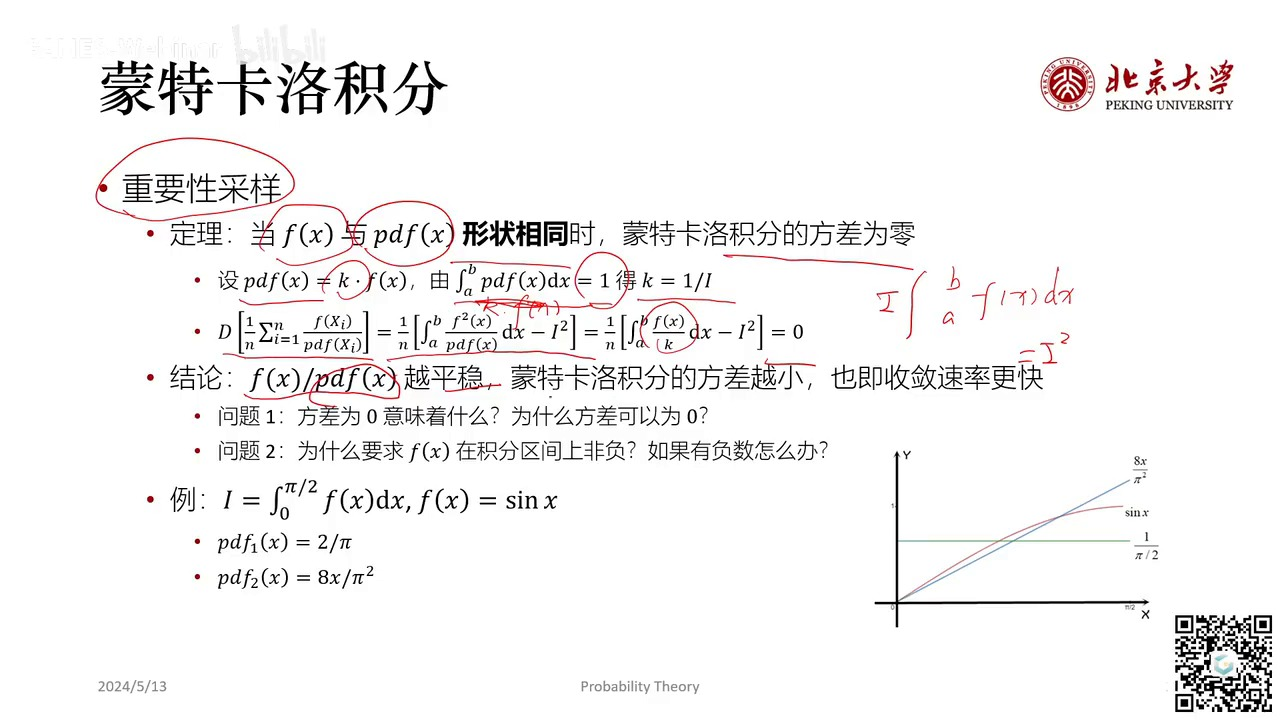
\includegraphics[width=0.92\textwidth]{figures/fig_13_importance.jpg}
\caption{重要性采样：形状相同时方差为零，以及 $\sin x$ 的例子\vtag}
\end{figure}
\srcnote{00:40:15--00:40:30}
\end{minipage}


\begin{importantbox}{重要性采样定理}
当 $f(x)$ 与 $\mathrm{pdf}(x)$ 形状相同时，蒙特卡洛积分的方差为零。设 $\mathrm{pdf}(x)=k\cdot f(x)$，由 $\int_a^b\mathrm{pdf}(x)\,\mathrm{d}x=1$ 得 $k=1/I$，代入方差公式，
\begin{equation}
D=\frac{1}{n}\left[\int_a^b\frac{f(x)}{k}\mathrm{d}x-I^2\right]=\frac{1}{n}\left[I^2-I^2\right]=0 .
\end{equation}
结论：$f(x)/\mathrm{pdf}(x)$ 越平稳，最好是一条水平线，蒙特卡洛积分的方差越小，收敛速率越快。
\end{importantbox}

\noindent\begin{minipage}{\textwidth}
\begin{figure}[H]
\centering
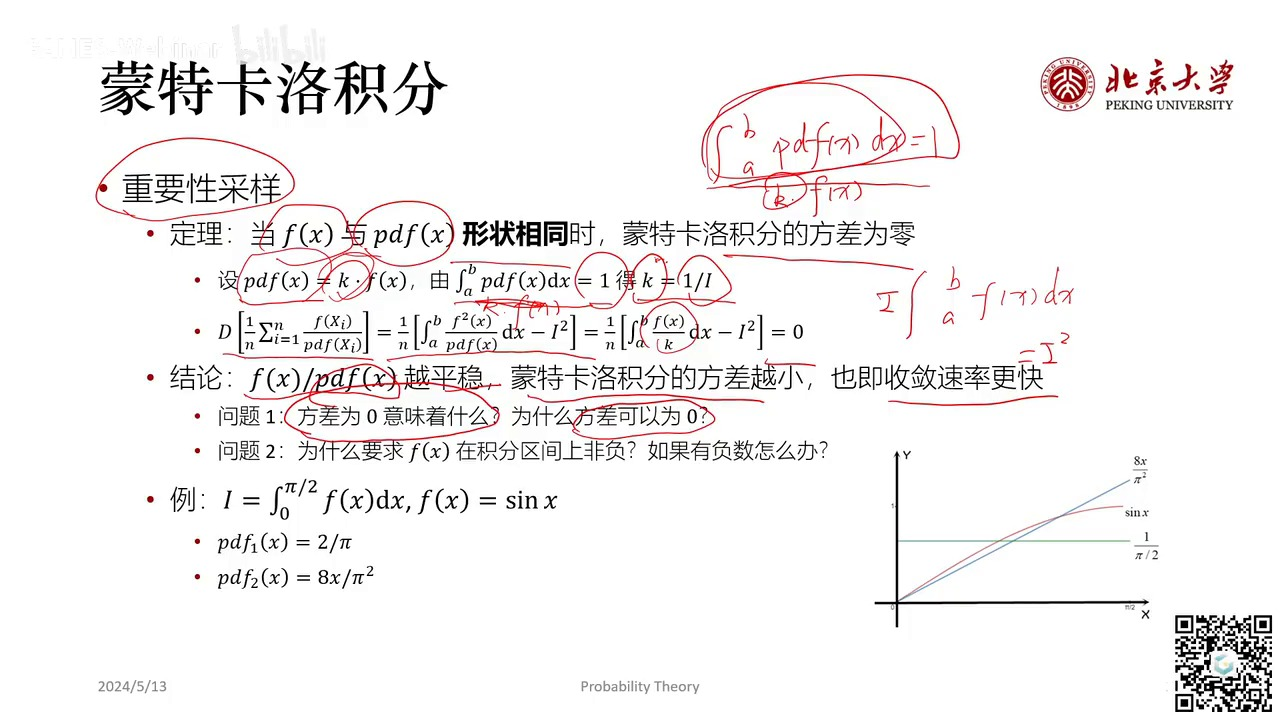
\includegraphics[width=0.92\textwidth]{figures/fig_14_importance_note.jpg}
\caption{讲者对“方差为零意味着什么”的批注\vtag}
\end{figure}
\srcnote{00:42:15--00:42:30}
\end{minipage}


\subsection{两个问题}

讲者提出了这个结论带来的两个问题。

\textbf{问题一：方差为零意味着什么？为什么方差可以为零？}要求 $f(x)$ 与 $\mathrm{pdf}(x)$ 形状相同，就意味着二者成正比，而要知道比例系数 $k$，就得先算出 $k=1/I$。换句话说，但凡你拿到了一个与 $f(x)$ 形状相同的概率密度，你一定已经把积分算出来了，结果是已知的，所以方差当然可以为零。

\textbf{问题二：为什么要求 $f(x)$ 在积分区间上非负？如果有负数怎么办？}若 $f$ 有负值，与它形状相同的 $\mathrm{pdf}$ 就会在某些点取负，出现取点概率为负的情况，上述定理就不成立了。讲者说，被积函数有负数时怎样做重要性采样是一个开放问题，有一些图形学的文章专门讨论特定渲染场景里的做法。

\begin{knowledgebox}{实践中的重要性采样}
讲义作者补充：既然完美的 $\mathrm{pdf}$ 需要事先知道答案，实践中就找一个容易采样、形状又与 $f$ 接近的分布。在渲染方程中，被积函数是 BRDF、入射光和余弦项的乘积，常见做法是按 BRDF 或按余弦项采样，形状“大致相同”就能显著降低噪声。
\end{knowledgebox}

\subsection{一个例子}

\noindent\begin{minipage}{\textwidth}
\begin{figure}[H]
\centering
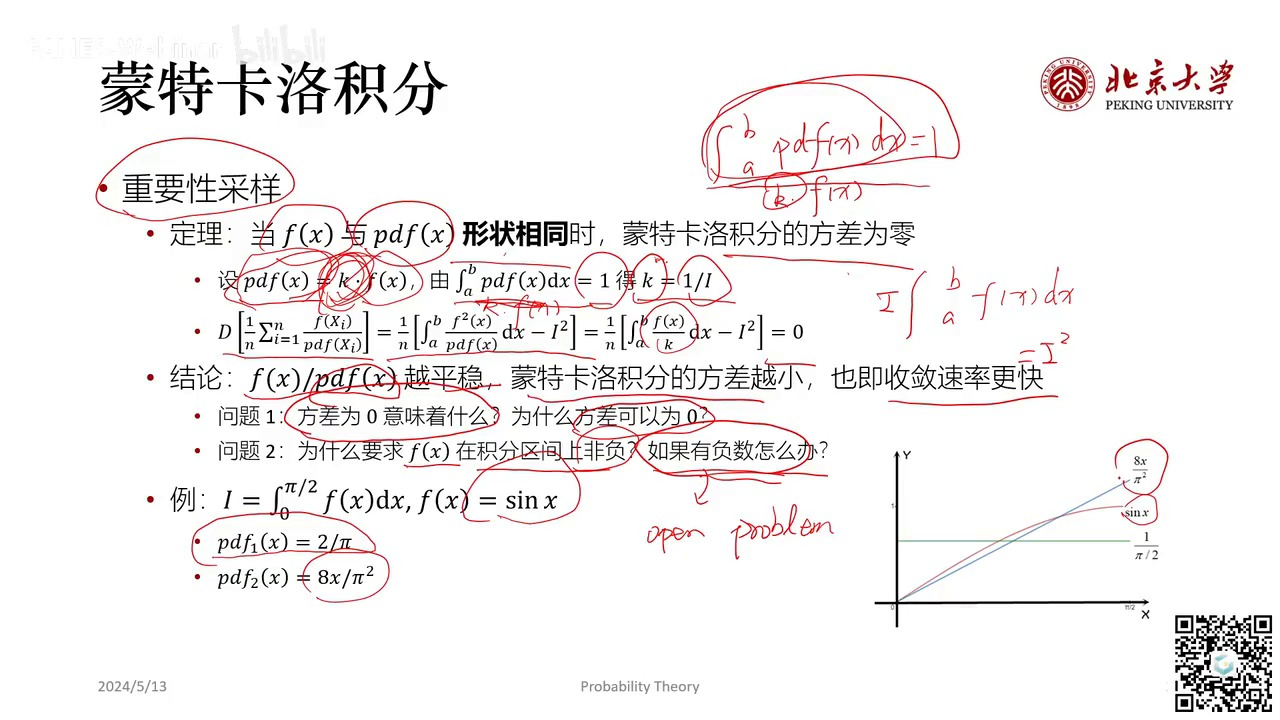
\includegraphics[width=0.92\textwidth]{figures/fig_15_importance_example.jpg}
\caption{$\sin x$ 与两种概率密度函数的图像\vtag}
\end{figure}
\srcnote{00:44:45--00:45:00}
\end{minipage}


考虑 $I=\int_0^{\pi/2}f(x)\,\mathrm{d}x$，$f(x)=\sin x$，即右图的红线。有两个不同的概率密度函数：第一个是 $[0,\pi/2]$ 上的均匀分布，第二个是一条过原点的斜线，在该区间上积分也为一：
\begin{equation}
\mathrm{pdf}_1(x)=\frac{2}{\pi},\qquad \mathrm{pdf}_2(x)=\frac{8x}{\pi^2}.
\end{equation}
从图上看，$\mathrm{pdf}_2$ 是一条过原点的斜线，与 $\sin x$ 的形状比水平线更接近，所以用它采样的方差更小。

\begin{practicebox}{算一算两种采样的方差}
读者可以用方差公式 $\int f^2/\mathrm{pdf}-I^2$ 验证（单样本，$I=1$；数值由讲义作者补算）：
\begin{enumerate}
\item 均匀分布：$\int_0^{\pi/2}\frac{\sin^2x}{2/\pi}\mathrm{d}x-1=\frac{\pi^2}{8}-1\approx 0.234$。
\item $\mathrm{pdf}_2=8x/\pi^2$：数值积分可得方差约为 $0.0167$，比均匀分布小一个数量级。
\end{enumerate}
\end{practicebox}

\section{拟蒙特卡洛法}

\subsection{分层采样}

\noindent\begin{minipage}{\textwidth}
\begin{figure}[H]
\centering
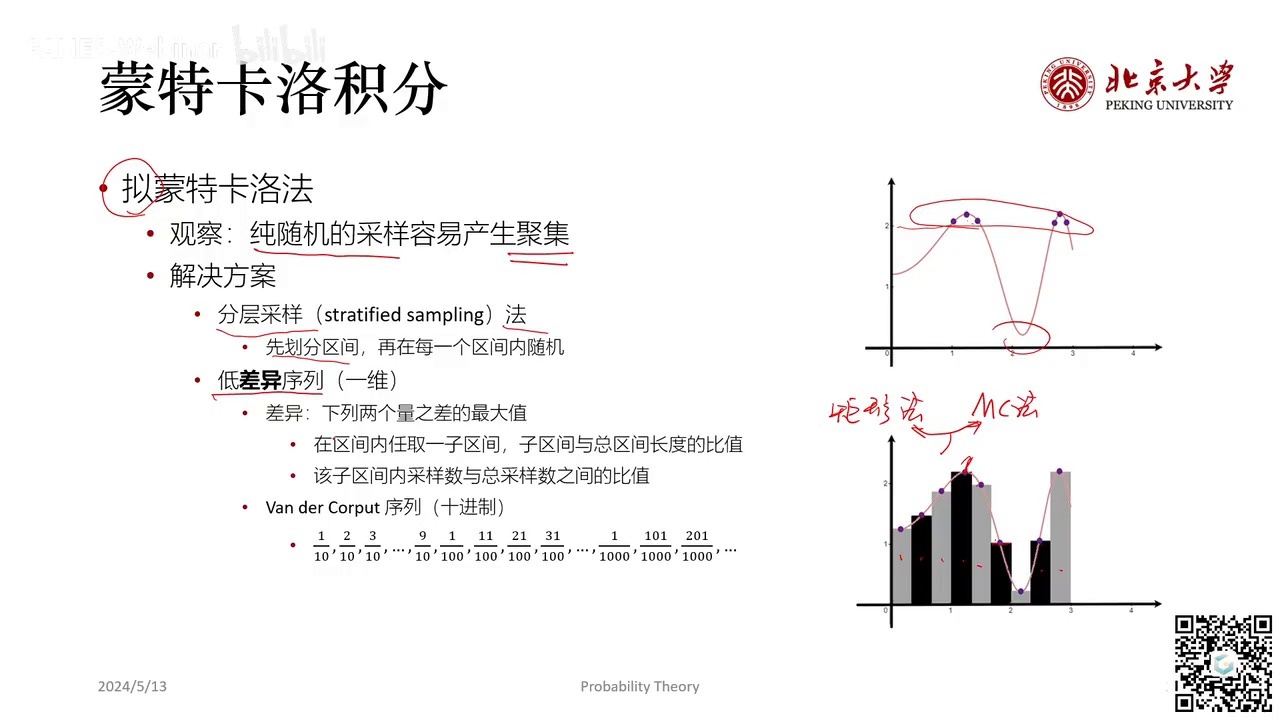
\includegraphics[width=0.92\textwidth]{figures/fig_16_qmc.jpg}
\caption{拟蒙特卡洛法：分层采样与一维低差异序列\vtag}
\end{figure}
\srcnote{00:47:00--00:47:15}
\end{minipage}


为什么叫“拟”蒙特卡洛法？因为蒙特卡洛法建立在纯随机的基础上，而纯随机的采样非常容易产生聚集。比如右图求一维积分，随机取的几个点可能挤在一起，函数在别处的变化就没有被采到。

第一种解决方案是分层采样（stratified sampling）：先分好子区间，再在每一个区间内随机取一点。讲者说这有点像回到了一开始估算定积分的矩形法，唯一的区别是：矩形法在每个区间内取固定位置，而分层采样在每个区间内随机取。

\subsection{低差异序列（一维）}

\noindent\begin{minipage}{\textwidth}
\begin{figure}[H]
\centering
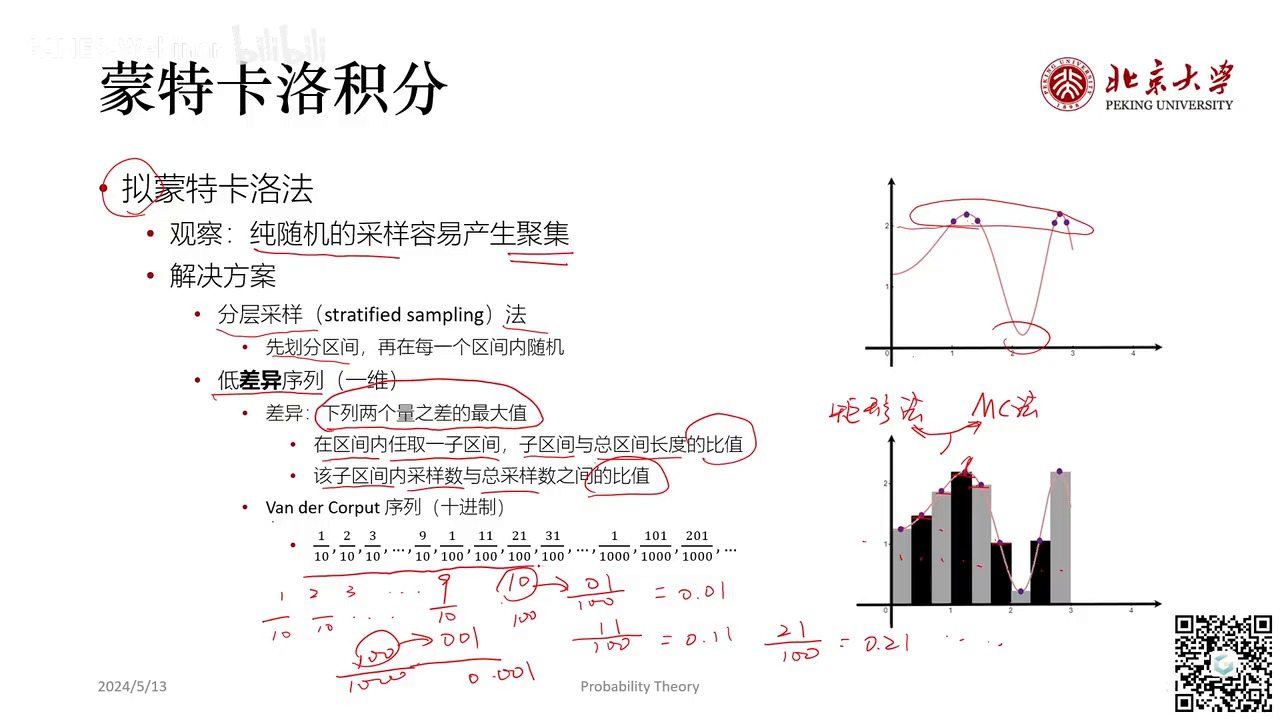
\includegraphics[width=0.92\textwidth]{figures/fig_17_vdc_note.jpg}
\caption{讲者演示 Van der Corput 序列的构造\vtag}
\end{figure}
\srcnote{00:49:45--00:50:00}
\end{minipage}


第二种方案是低差异序列。“差异”（discrepancy）是“聚集”的反义词式的度量：在积分区间内任取子区间，计算子区间与总区间长度的比值，以及该子区间内采样数与总采样数的比值，这两个量之差的最大值就是差异。低差异序列就是让这个差异尽可能小的序列，而纯随机的方法完全不保证这一点。讲者说，整个二十世纪大家研究随机算法时，已经发现了很多这样的低差异序列。

一维最简单的是 Van der Corput 序列。十进制下，它的构造方法非常简单：把正整数 $1,2,3,\dots$ 的各位数字顺序颠倒，放到小数点后面。例如 $1,2,\dots,9$ 依次给出 $0.1,0.2,\dots,0.9$；$10$ 颠倒为 $01$，给出 $1/100$；$11$ 的个位和十位一样，还是 $11/100$；$12$ 颠倒为 $21$，给出 $21/100$。课件上的序列为
\begin{equation}
\frac{1}{10},\frac{2}{10},\frac{3}{10},\dots,\frac{9}{10},\frac{1}{100},\frac{11}{100},\frac{21}{100},\frac{31}{100},\dots,\frac{1}{1000},\frac{101}{1000},\frac{201}{1000},\dots
\end{equation}
讲者指出它的另一个好处：算法是迭代的，长度为 $101$ 的序列就是在长度为 $100$ 的序列后面补一个数，使用非常方便。

\begin{warningbox}{课件上的数字}
讲者口头说“$11$ 的个位和十位一样，所以还是产生零点一”，这里口误了：$11$ 颠倒后仍是 $11$，对应的是 $11/100=0.11$，与课件上的序列一致。
\end{warningbox}

\subsection{高维：Halton 与 Hammersley 序列}

\noindent\begin{minipage}{\textwidth}
\begin{figure}[H]
\centering
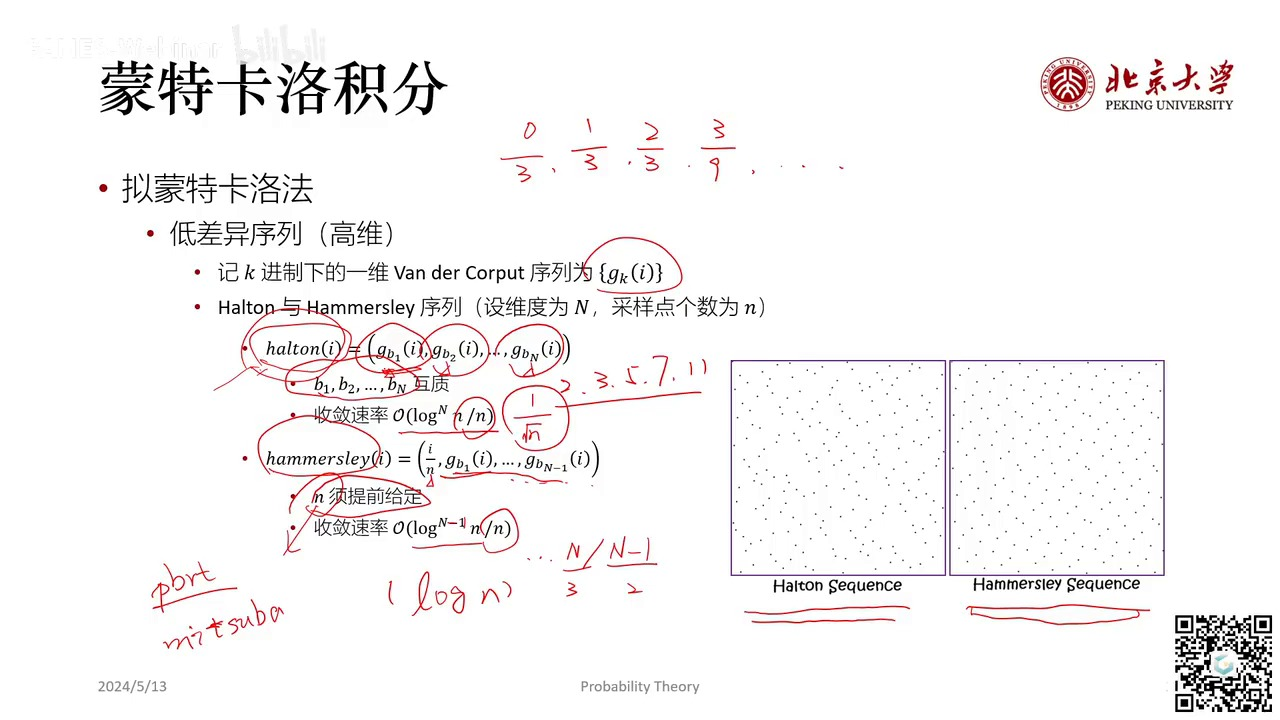
\includegraphics[width=0.92\textwidth]{figures/fig_18_halton.jpg}
\caption{高维低差异序列：Halton 序列与 Hammersley 序列\vtag}
\end{figure}
\srcnote{00:54:15--00:54:30}
\end{minipage}


记 $k$ 进制下的一维 Van der Corput 序列为 $\{g_k(i)\}$。设维度为 $N$，采样点个数为 $n$。Halton 序列取 $N$ 个两两互质的进制底数 $b_1,b_2,\dots,b_N$，比如取质数序列 $2,3,5,7,\dots$，令
\begin{equation}
\mathrm{halton}(i)=\left(g_{b_1}(i),g_{b_2}(i),\dots,g_{b_N}(i)\right),
\end{equation}
收敛速率为 $O(\log^N n/n)$。讲者强调，用这种序列而不是纯随机方法采样，收敛速率是以 $n$ 分之一为底，而不是前面说的 $1/\sqrt n$，快了很多。

Hammersley 序列的唯一区别在于：把第一维换成 $i/n$，即
\begin{equation}
\mathrm{hammersley}(i)=\left(\frac{i}{n},g_{b_1}(i),\dots,g_{b_{N-1}}(i)\right).
\end{equation}
它要求 $n$ 必须提前给定，收敛速率为 $O(\log^{N-1}n/n)$，分子的次幂比 Halton 降了一次。从右图看，它比 Halton 序列差异更小一些、聚集更少、更均匀。讲者说，真正实现渲染算法时，基本上用的都是这类序列产生的“随机数”，优势就在于此。

\begin{knowledgebox}{序列维度 $N$ 的影响}
讲义作者补充：$O(\log^N n/n)$ 中的 $\log^N n$ 随维度增长很快，所以在维度很高时，低差异序列相对纯随机的优势会变小。路径追踪中一条路径的维度很高，实践中常把它拆成多个低维片段分别使用低差异序列。
\end{knowledgebox}

\section{随机数的变换：在球面上均匀采样}

\subsection{问题}

\noindent\begin{minipage}{\textwidth}
\begin{figure}[H]
\centering
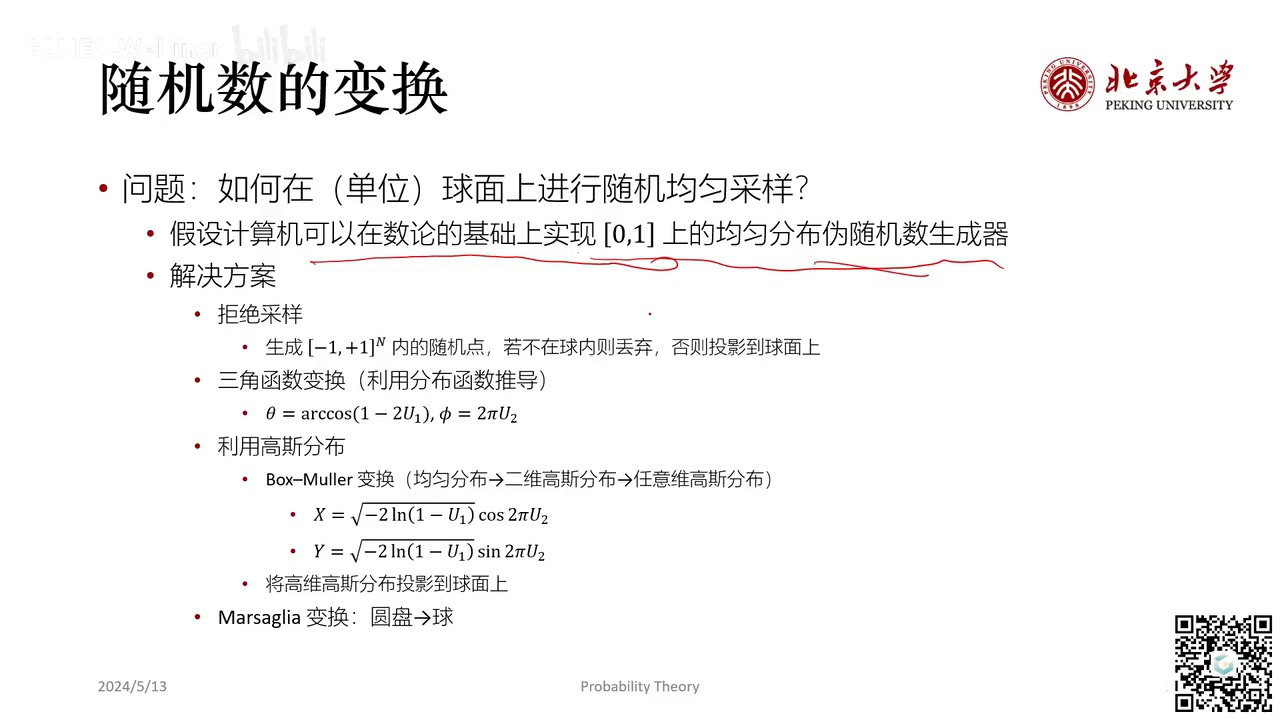
\includegraphics[width=0.92\textwidth]{figures/fig_19_sphere.jpg}
\caption{随机数的变换：在单位球面上均匀采样的四种方案\vtag}
\end{figure}
\srcnote{00:54:45--00:55:00}
\end{minipage}


最后的问题是：如何在单位球面上进行随机均匀采样？讲者说这个问题蛮重要：比如做路径追踪时，有入射角和出射角，需要在半球面上采样，并且希望采样尽可能均匀。假设计算机可以在数论的基础上实现 $[0,1]$ 上的均匀分布伪随机数生成器，记生成的随机数为 $U_1,U_2,\dots$。

\subsection{方案一：拒绝采样}

生成 $[-1,+1]^N$ 内的随机点，若不在球内则丢弃，否则投影到球面上。以二维为例，正方形内每个点的坐标由两个随机数组成，直接用随机数生成器生成即可；若点落在圆内就保留，相当于生成了圆内均匀的随机点，再把它从圆心投影到圆周上，就能保证最后生成单位圆上的均匀点。

\subsection{方案二：三角函数变换}

利用分布函数推导。三维球面上的点一般用球坐标表示，有两个角 $\theta$ 和 $\phi$。要看的是：改变 $\theta$ 会增加多少面积，改变 $\phi$ 又会增加多少面积。

\noindent\begin{minipage}{\textwidth}
\begin{figure}[H]
\centering
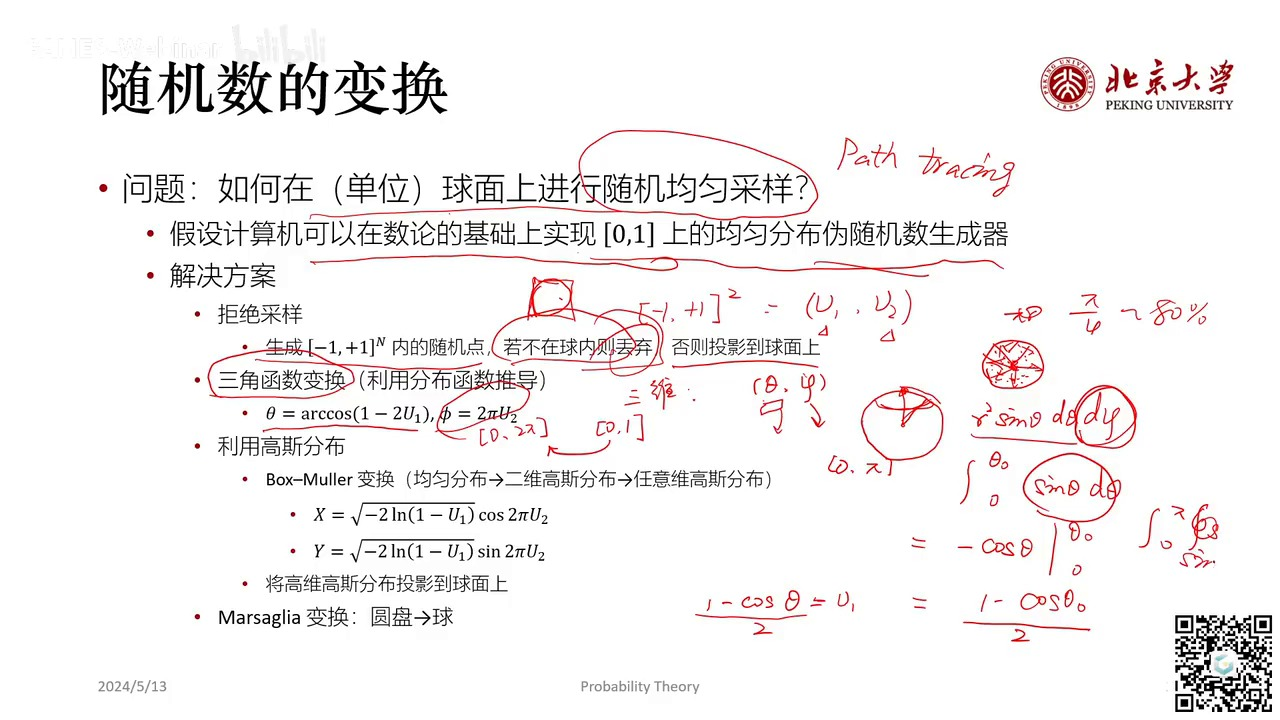
\includegraphics[width=0.92\textwidth]{figures/fig_20_sphere_note.jpg}
\caption{讲者推导 $\theta$ 的分布函数\vtag}
\end{figure}
\srcnote{01:01:00--01:01:15}
\end{minipage}


对 $\phi$：不管 $\phi$ 取多少，概率密度都一样，$\phi$ 可以取 $0$ 到 $2\pi$，而 $U_2$ 是 $[0,1]$ 上的随机数，所以直接取 $\phi=2\pi U_2$。对 $\theta$：从球坐标的顶开始往下到 $\theta_0$，扫过的球冠面积与 $1-\cos\theta_0$ 成正比；对 $\theta$ 从 $0$ 到 $\pi$ 积分得到 $2$，为了归一化要乘以 $1/2$，于是分布函数为
\begin{equation}
F(\theta_0)=\frac{1}{2}\left(1-\cos\theta_0\right).
\end{equation}
令它等于随机数 $U_1$，变换一下就得到
\begin{equation}
\theta=\arccos(1-2U_1),\qquad \phi=2\pi U_2 .
\end{equation}

\begin{warningbox}{不要直接均匀取两个角}
讲义作者提醒：若直接令 $\theta=\pi U_1$，点会在两极聚集，因为靠近两极的纬圈很短，同样的 $\Delta\theta$ 对应的面积小。上式中的 $\arccos$ 正是为了按面积而不是按角度均匀。
\end{warningbox}

\subsection{方案三：利用高斯分布}

高斯分布有非常好的性质：二维高斯分布在任何方向上看都是高斯分布，它是旋转对称的。所以把高维的高斯分布投影到球面上，得到的依然是均匀分布。讲者说这个方法很巧妙，但它唯一的问题在于生成高斯分布本身并不容易，需要用 Box--Muller 变换，从均匀分布到二维高斯分布，再到任意维高斯分布。设 $U_1,U_2$ 是 $[0,1]$ 上的随机变量，
\begin{equation}
\begin{gathered}
X=\sqrt{-2\ln(1-U_1)}\cos 2\pi U_2,\\
Y=\sqrt{-2\ln(1-U_1)}\sin 2\pi U_2 .
\end{gathered}
\end{equation}
然后将高维高斯分布投影到球面上。

\subsection{方案四：Marsaglia 变换}

最后一种是 Marsaglia 变换：从圆盘映射到球面。讲者说这个过程的好处是从头到尾不涉及三角函数运算。三角函数方法需要 $\arccos$、$\cos$、$\sin$，而圆盘到球的方法不产生任何三角函数运算，所以速度反而很快。

\noindent\begin{minipage}{\textwidth}
\begin{figure}[H]
\centering
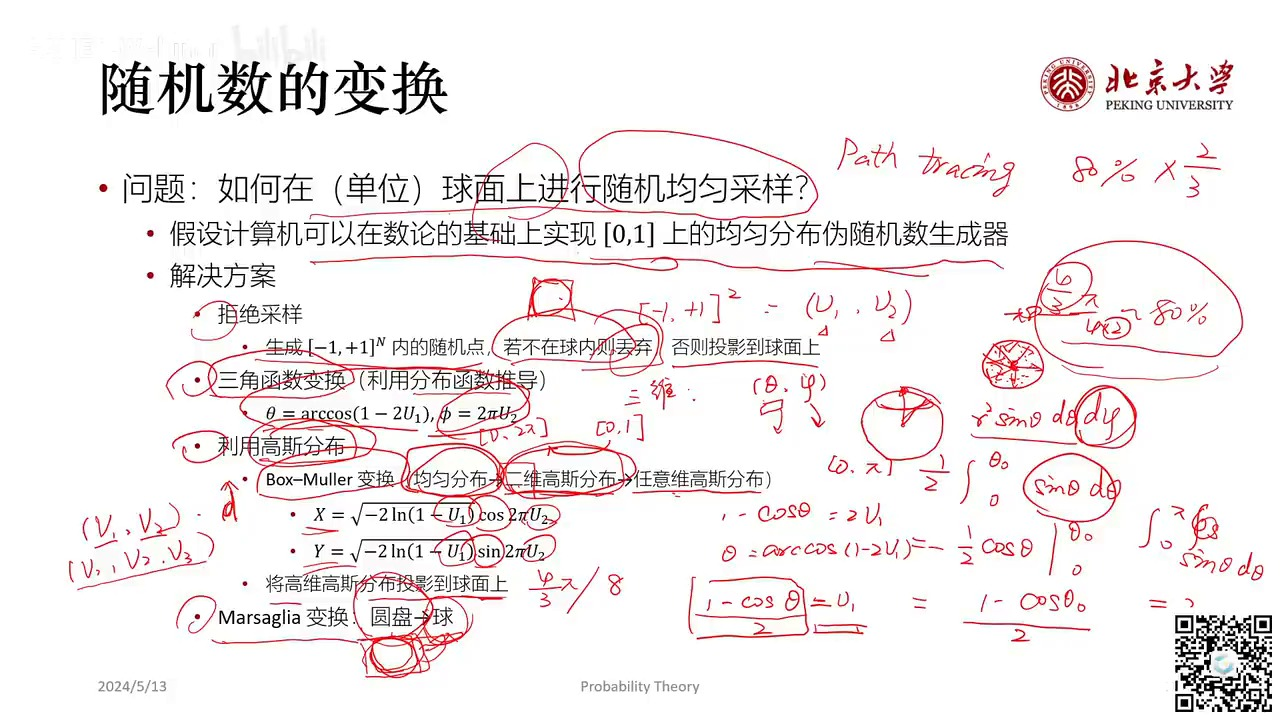
\includegraphics[width=0.92\textwidth]{figures/fig_21_sphere_note2.jpg}
\caption{讲者比较拒绝采样在二维与三维中的接受率\vtag}
\end{figure}
\srcnote{01:08:00--01:08:15}
\end{minipage}


讲者顺便比较了拒绝采样的效率。二维时，正方形内的点落在圆内的概率约为百分之八十；三维时，分母上体积乘了 $2$，分子上却只乘了 $4/3$，概率再乘以 $2/3$，只剩约一半。Marsaglia 方法只需要在圆盘上做拒绝采样，扔掉的点比直接在球内生成随机数要少得多。

\begin{practicebox}{核对接受率}
讲义作者补充精确值：二维时圆与外接正方形面积比为 $\pi/4\approx 78.5\%$；三维时球与外接立方体体积比为 $\pi/6\approx 52.4\%$，正好是二维值乘以 $2/3$。维度再升高，接受率会迅速趋于零，这也是高维时不宜用拒绝采样的原因。
\end{practicebox}

\section{小结}

讲者说，几种思路中第二、三种的实现细节已经给出，照抄式子就可以；第四种映射方法式子比较长，大家可以自己去查。下节课的内容是场论初步。

回顾本讲：噪声的“颜色”由频谱决定；图像抖动通过加噪声让二值化结果在期望上等于原亮度，蓝噪声最符合人眼；蒙特卡洛积分是无偏估计，误差按 $1/\sqrt n$ 下降，重要性采样通过让 $\mathrm{pdf}$ 贴近被积函数来降低方差，低差异序列通过让样本更均匀来加快收敛；最后，在球面上均匀采样需要按面积而不是按角度变换随机数。

\begin{knowledgebox}{与上一讲的联系}
本讲用到的工具都来自上一讲：抖动的分析用的是期望，蒙特卡洛积分的无偏性和 $1/\sqrt n$ 误差来自期望和方差的性质，而撒点求面积的收敛性直接来自伯努利大数定律。
\end{knowledgebox}

\end{document}
